\documentclass[a4paper,twocolumn,10pt]{article}
%\usepackage[dvips]{graphicx}      % どっちかを使う(こっちを使うとepsがずれる)
\usepackage[dvipdfmx]{graphicx}   % どっちかを使う
\usepackage{here}     % 表や図の位置を固定するhereを使用可にする
\usepackage{amsmath}  % 複雑な数式用
\usepackage{amssymb}  % 複雑な数式用
\usepackage{bm}
\usepackage[subrefformat=parens]{subcaption}
\newcommand{\argmin}{\mathop{\rm arg~min}\limits}
%
% sectionの字を小さくする
\makeatletter
\renewcommand{\section}{%
  \@startsection{section}%
   {1}%
   {\z@}%
   {0ex \@plus -1ex \@minus -.2ex}%
   {2.3ex \@plus.2ex}%
   {\normalfont\large\bfseries}%
}%
\makeatother
%
% 余白の調整 (A4用紙は595ptx842pt)
% 左側の余白
\setlength{\oddsidemargin}{-20pt}
% 本文テキスト全体の幅
\setlength{\textwidth}{510pt}
% 上側の余白
\setlength{\topmargin}{-40pt}
% ヘッダの高さ
\setlength{\headheight}{0pt}
% ヘッダと本文テキストとの間の余白
\setlength{\headsep}{0pt}
% 本文テキスト全体の高さ
\setlength{\textheight}{780pt}
%
\begin{document}
% このページのスタイルを指定 - ヘッダ・フッタなし
\thispagestyle{empty}
%
\twocolumn[
\begin{center}
\Large \textbf{Low-Light Image Enhancement via Mixture $L_{2}$ - $L_{p}$ Variational Retinex Model with Adaptive Texture Map}
\end{center}
\vspace{-3mm}
\begin{center}
\begin{large}
Student ID:29C18023 ~ ~ Iiguni Lab. ~ ~ Kazuki Kurihara
\end{large}
\end{center}
]
% 行間の指定
\setlength{\baselineskip}{3mm}
%
\section{Introduction}
\thispagestyle{empty}
\vspace{-0.3cm}
The methods of low-light image enhancement have been paid attention to with the wide spread of computer vision applications used in outdoors. We develop a mixture $L_{2}$ - $L_{p}$ variational model with an adaptive texture map in order to enhance low-light images naturally. We evaluate the effectiveness of the proposed method both qualitatively and quantitatively.
\vspace{0.1cm}
\section{Variational Retinex Model}
\vspace{-0.3cm}
The Retinex theory \cite{retinex} is a color perception model based on human visual system. 
The model decomposes an observed image into reflectance and illumination as follows:
\vspace{-0.3cm}
\begin{eqnarray}
S = R \circ I, \label{eq:retinex}
\vspace{-0.3cm}
\end{eqnarray}
where $S$, $R$, and $I$ represent an observed image, reflectance, and illumination, respectively. Reflectance represents the intrinsic characteristics of the object, while illumination represents the extrinsic property.\par 
Cai $et$ $al.$ \cite{jiep} proposed a variational optimization-based Retinex model using the local variation deviation (LVD) as the constraint term on illumination:
\vspace{-0.25cm}
\begin{eqnarray}
	\begin{split}
		&\argmin_{R, I} \|R \circ I - S\|_{2}^{2} + \alpha{\left \|\frac{\nabla{I}}{\frac{1}{|\Omega|}\Sigma_{\Omega}\nabla{I} + \epsilon} \right\|_{1}}\\
		&+ \beta{\|\nabla{R}\|_{1}} + \gamma{\|I - B\|_{2}^{2}}.
	\end{split}
\end{eqnarray}
Since the LVD sufficiently distinguishes between texture and structure, this method can smooth illumination while keeping the structure information.
\vspace{0.1cm}
\section{$L_{2}$ - $L_{p}$ Variational Retinex Model \\ with Adaptive Texture Map}
\vspace{-0.3cm}
The proposed method develops a mixture $L_{2}$ - $L_{p}$ variational optimization-based Retinex model which introduces $L_{2}$ and $L_{p}$ norms into the constraint terms on reflectance and illumination in the cost function:
\vspace{-0.25cm}
\begin{eqnarray}
\begin{split}
	&\argmin_{R, I} \|R \circ I - S\|_{2}^{2} + \alpha \left \|\frac{\nabla{I}}{\frac{1}{|\Omega|}\Sigma_{\Omega}\nabla{I}+\epsilon}\right\|_{p}^{p} \\
	& + \beta \|W \circ \nabla{R}\|_{2}^{2} + \gamma \|I - B\|_{2}^{2}, \label{eq:proposed/equation}
\end{split}
\vspace{-0.1cm}
\end{eqnarray}
where $\| \cdot \|_{p}$ denotes a $L_{p}$ norm constraint term $(0 \leq p \leq 2)$ on illumination, and $W$ represents an adaptive texture map which is the weight of the constraint term on reflectance in order to preserve more textures detail while reducing noise in the estimated reflectance.\par 
Since the $L_{p}$ constraint term causes non-smooth optimization, the proposed method adopts an iteratively re-weighted least square (IRLS) and rewrite the second term in the function $(\ref{eq:proposed/equation})$ as follows:
\vspace{-0.2cm}
\begin{eqnarray}
\left \|\frac{\nabla{I}}{\frac{1}{|\Omega|}\Sigma_{\Omega}\nabla{I}+\epsilon}\right\|^{p} = \|U \circ \nabla{I}\|^{2}, \label{eq:approximation}
\end{eqnarray}
\vspace{-0.5cm}
\begin{align}
U &= \left \{
  	\begin{array}{ll}
  	\frac{1}{\xi^{2-p}}, 
  	& \left |\frac{\nabla{I}}{\frac{1}{|\Omega|} \sum_{\Omega} \nabla{I} } \right| < \xi\\
  	\frac{1}{\left |\frac{1}{|\Omega|}\Sigma_{\Omega} \nabla{I} \right|^{p} \left |\nabla{I} \right|^{2-p}},
  	& \rm{otherwise}
  	\end{array}
\right. . \label{eq:lp_shape}
\end{align}\par
Moreover, the adaptive texture map $W$ is set so that the map adaptively assigns different values to dark and bright according to the brightness of an observed image. In addition, the map contributes to reveal fine textures detail in the estimated reflectance. The map is formulated as:
\vspace{-0.3cm}
\begin{eqnarray}
W = \frac{1.0 - \max_{c \in \{r, g, b\}}{S_{c}}}{\left |\frac{1}{|\Omega|}\sum_{\Omega}\nabla{R} \right|^{a_{r}} + \epsilon}, \label{eq:proposed/adaptive}
\end{eqnarray}
\vspace{-0.4cm}
\begin{eqnarray}
a_{r} = 1.0 - |\nabla{R}|\exp(1.0 - |\nabla{R}|), \label{eq:adaptive/parameter}
\end{eqnarray}
where $a_{r}$ $(0 \leq a_{r} \leq 1)$ represents an exponential parameter to adjust the awareness of textures detail for reflectance. The smaller the parameter $a_{r}$ is, the more reveled the edges and textures detail are in the estimated reflectance. On the other, the larger the parameter is, the more smoothed the flat and homogeneous regions are in the estimated reflectance.
\vspace{0.1cm}
\section{Experiments}
\vspace{-0.3cm}
We conducted both qualitative and quantitative evaluations. In the qualitative evaluation, as shown in Fig.\ref{fig:qualitative}, we can see that the proposed method significantly enhances the low-light image while suppressing noise amplification and over-enhancement. Moreover, Fig.\ref{fig:quantitative} summarizes the results of the quantitative evaluations to indicate the naturalness of the enhanced images: lightness order error (LOE) and autoregressive-based image sharpness metric (ARISM). We can see that the proposed method achieves the best performances in both quantitative evaluations.
%----定性評価---- %
\begin{figure}[tb]
	\begin{tabular}{cc}
      \begin{minipage}{0.5\hsize}
        \begin{center}
 			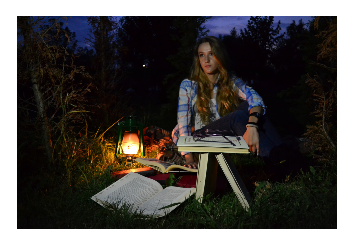
\includegraphics[width=\hsize]{images/qualitative/input.eps}
			 \subcaption{Observed image.}
        \end{center}
      \end{minipage}
      \begin{minipage}{0.5\hsize}
        \begin{center}
 			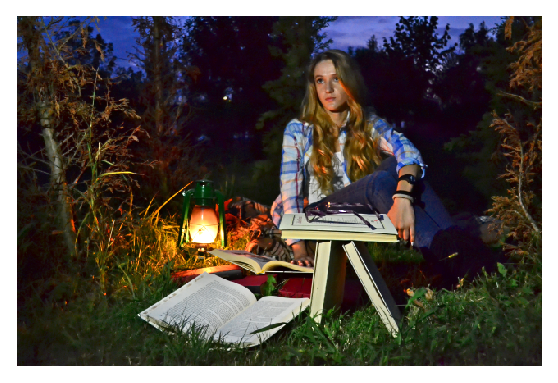
\includegraphics[width=\hsize]{images/qualitative/output.eps}
 			\subcaption{Enhanced image.}
        \end{center}
      \end{minipage}
	\end{tabular}
	\caption{The enhanced image by the proposed method.}
	\label{fig:qualitative}
	\vspace{-0.3cm}
\end{figure}
%----定量評価---- %
\begin{figure}[tb]
	\begin{tabular}{cc}
      \begin{minipage}{0.5\hsize}
        \begin{center}
 			
\includegraphics[width=\hsize]{images/quantitative/loe.eps}
			 \subcaption{LOEs.}
        \end{center}
      \end{minipage}
      \begin{minipage}{0.5\hsize}
        \begin{center}
 			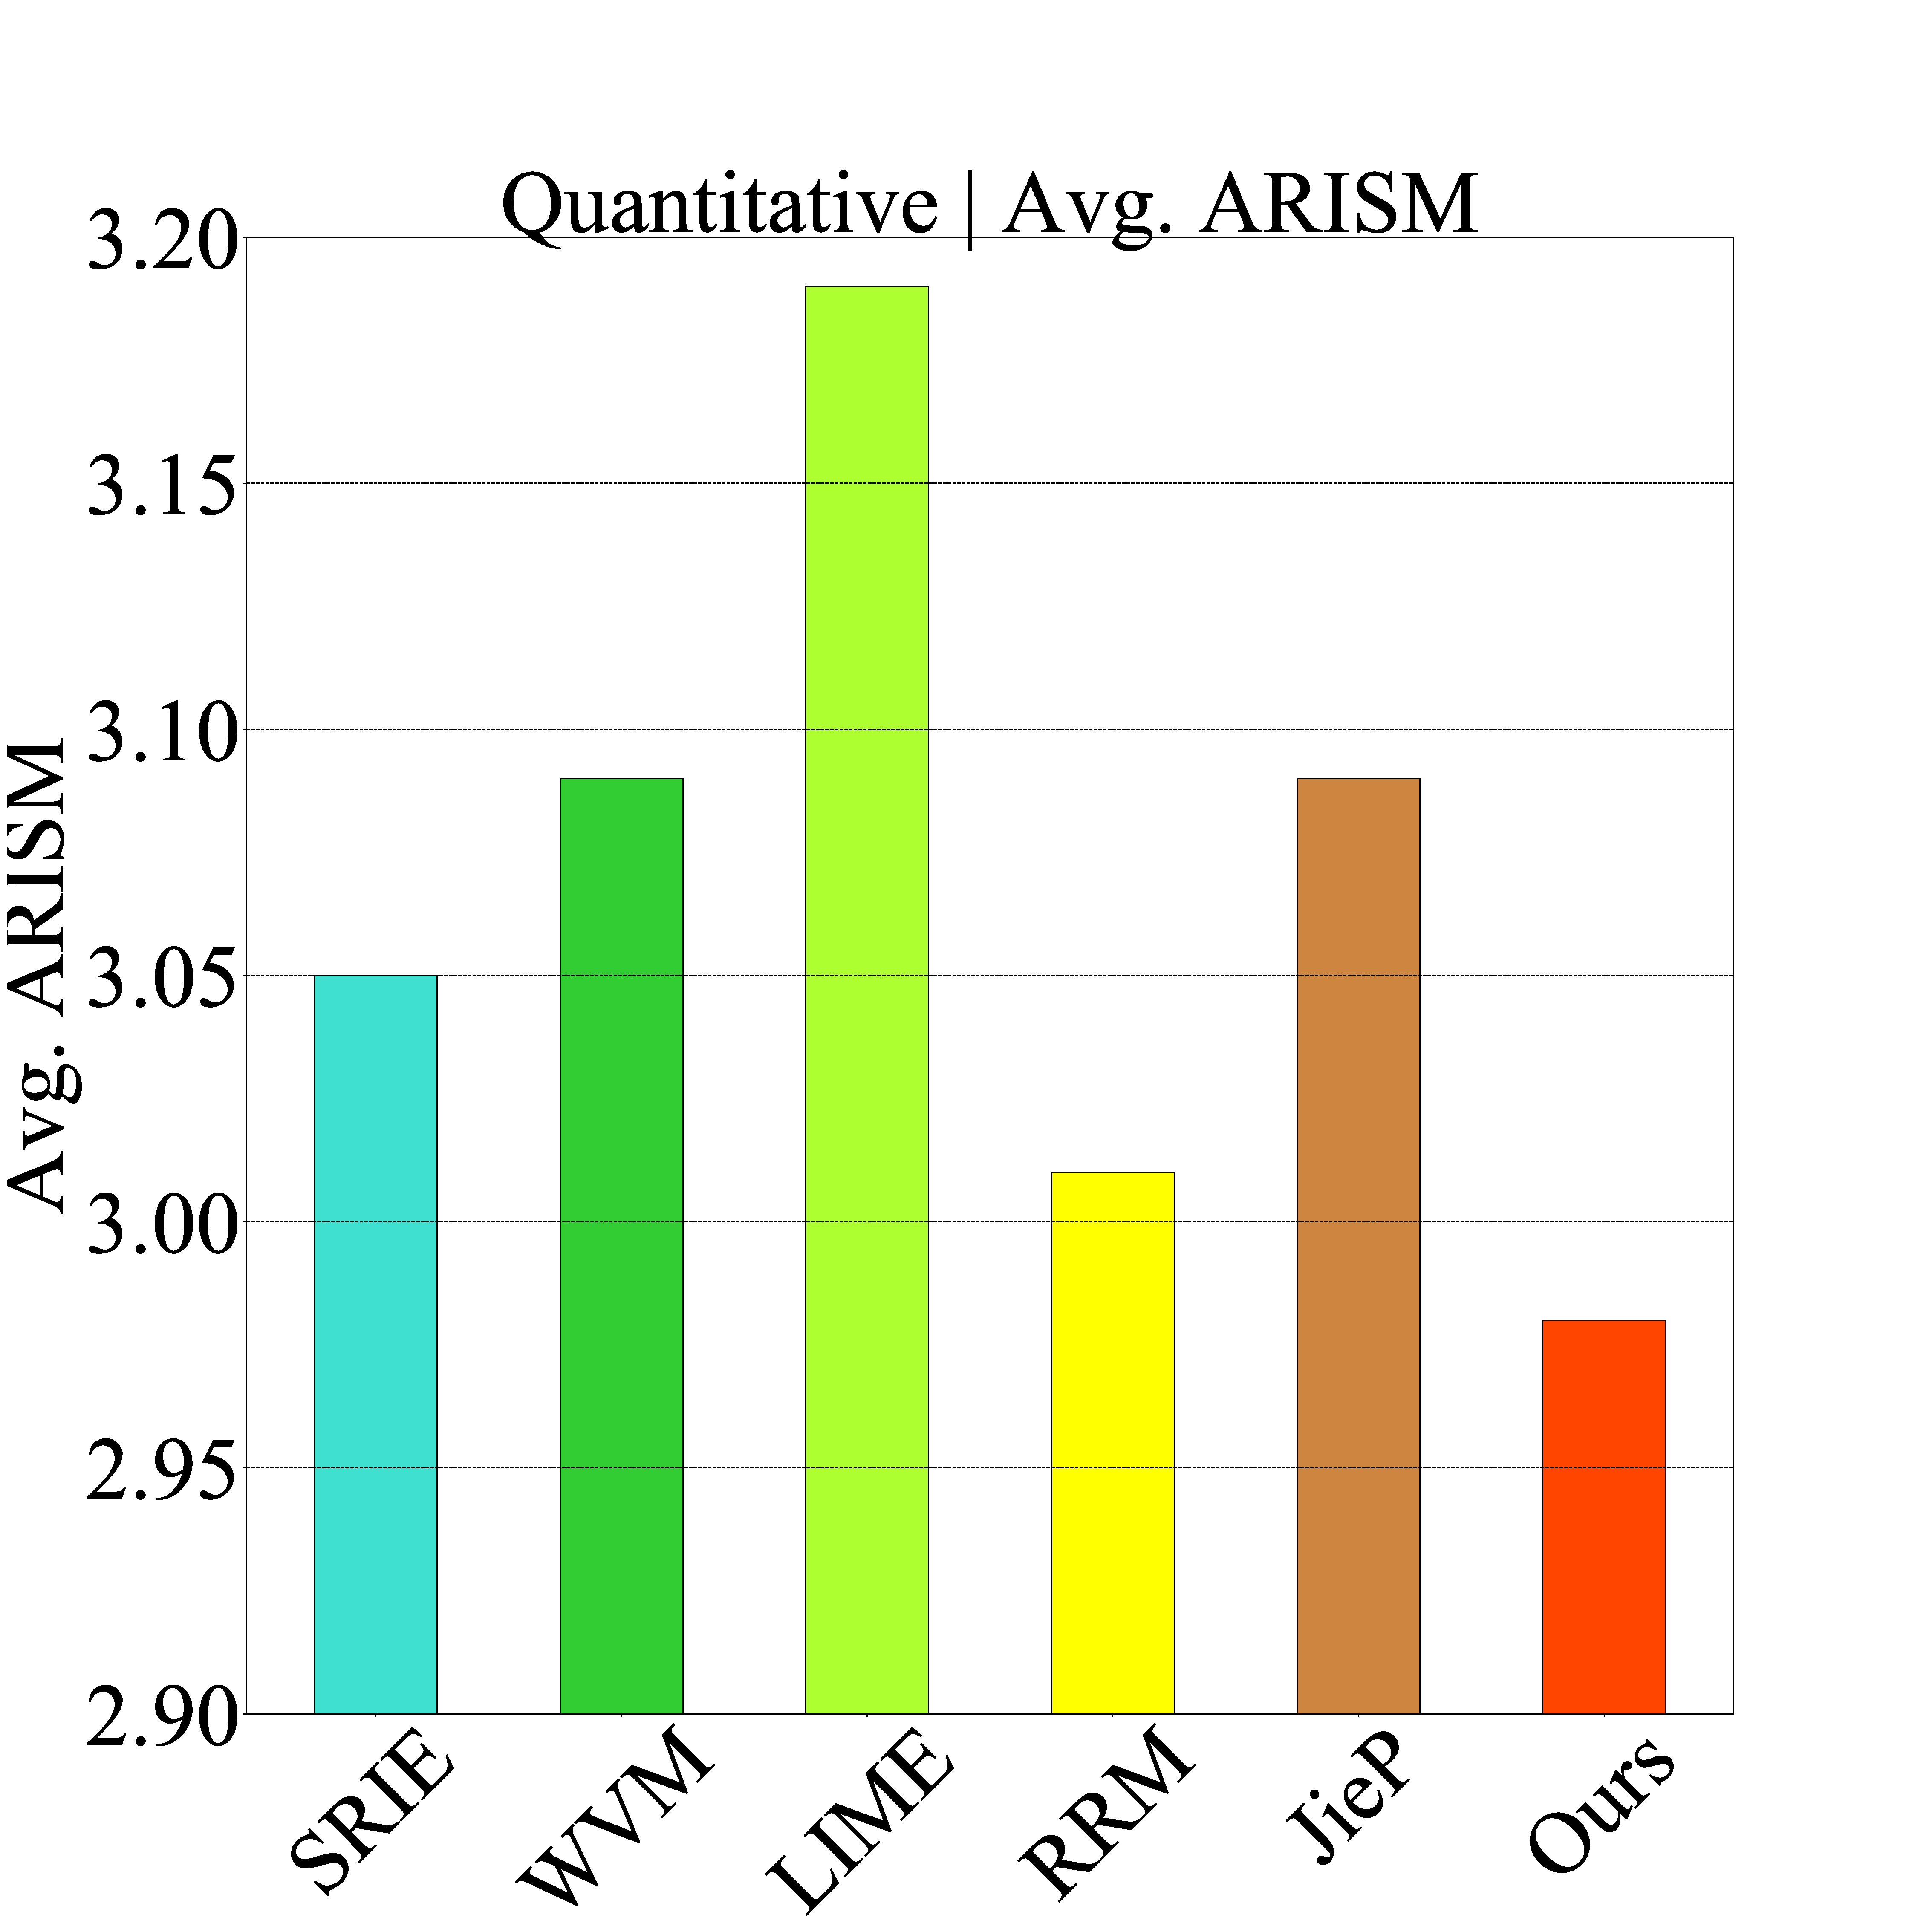
\includegraphics[width=\hsize]{images/quantitative/arism.eps}
 			\subcaption{ARISMs.}
        \end{center}
      \end{minipage}
	\end{tabular}
	\caption{Plots of the results of different quantitative evaluations for all the competing methods.}
	\label{fig:quantitative}
	\vspace{-0.5cm}
\end{figure}
\section{Conclusion and Future Works}
\vspace{-0.3cm}
This paper developed the mixture $L_{2}$ - $L_{p}$ variational Retinex model with the adaptive texture map.
We showed that the proposed method outperformed the other methods in terms of the indicators of naturalness.
In the future work, we have to create pseudo-darken images and evaluate the proposed method with such images.
\vspace{0.1cm}
\begin{thebibliography}{9}
\vspace{-0.2cm}
\bibitem{retinex} E. H. Land and J. J. McCann, ``Lightness and retinex theory,'' JOSA, vol.61, no.1, pp.1-11, 1971.
\vspace{-0.1cm}
\bibitem{jiep} B. Cai, X. Xu, K. Guo, K. Jia, B. Hu, and D. Tao, ``A joint intrinsic-extrinsic prior model for retinex,'' Proc. of IEEE Conf. Computer Vision, Pattern Recog., pp.4000-4009, 2017.
\end{thebibliography}

\end{document}
